\section{Pseudocode & Algoritmes}

\begin{frame}
\frametitle{Hoe zet je een probleem om in een programma?}

\begin{itemize}
  \item<1-> Begin met het probleem te versimpelen.
  \item<2-> Denk vervolgens als een computer:
  \begin{itemize}
  	\item<3-> Niets is ``duidelijk'' of ``obvious'': 
	  \begin{itemize}
	  	\item<4-> De computer denkt niet zelf na!
	  \end{itemize}
  	\item<5-> Je moet alles letterlijk uitspellen voor de computer!
  \end{itemize}
  \item<6-> Het helpt om gebruik te maken van ``pseudocode''.
\end{itemize}

\end{frame}



\begin{frame}
\frametitle{Wat is pseudocode?}

\begin{itemize}
  \item<1-> Pseudocode ligt tussen ``echte'' code en mensentaal in.
  \begin{itemize}
  	\item<2-> ``Echte'' code heeft een strakke syntax waar je je aan moet houden.
  	\begin{itemize}
  	  \item<3-> Een kleine typefout en de computer begrijpt je niet!
  	\end{itemize}
  	\item<4-> Pseudocode heeft niet zo'n strakke syntax,\\maar het is ``in eigen woorden''
  \end{itemize}
  \item<5-> Pseudocode heeft echter wel de \textbf{structuur} van een algoritme
\end{itemize}

\end{frame}




\begin{frame}
\frametitle{Wat is pseudocode?}
\framesubtitle{Voorbeeld}

Stel dat we een programma willen schrijven die ons vertelt of we vandaag een paraplu nodig hebben.
\visible<2>{In pseudocode:}


\visible<2->{
\begin{minipage}{0.7\textwidth}%
	\begin{algorithm}[H]
	\caption{Pseudocode ``paraplu nodig?''}
	\begin{algorithmic}[1]
	\Function{ParapluNodig}{regenkans}
	   \If{regenkans = hoog}
	     \State Paraplu nodig
	   \ElsIf{regenkans = laag}
	     \State Geen paraplu nodig
	   \Else
	     \State Paraplu optioneel. \Comment{Je smelt niet!}
	   \EndIf
	\EndFunction
	\end{algorithmic}
	\end{algorithm}
\end{minipage}%
\visible<3->{
\begin{minipage}{0.27\textwidth}%
	\begin{ticalc}
		PROGRAM\:PARAPLU\\%
		\:If\,R>40\\%
		\:Then\\%
		\:Disp\,\qt PARAPLU\,NODIG\qt\\%
		\:Else\:If\,R<10\\%
		\:Then\\%
		\:Disp\,\qt PARAPLU\,ONNODIG\qt\\%
		\:Else\\%
		\:Disp\,\qt PARAPLU\,OPTIONEEL\qt\\%
		\:End
		\:End
	\end{ticalc}
\end{minipage}%	
}
}


\addtocounter{algorithm}{-1} % Prevents the algorithm number to increase every frame
\end{frame}
\addtocounter{algorithm}{1} % Make sure the number increases for a new algorithm on a different slide


\begin{frame}
\frametitle{Wat is het nut van pseudocode?}

Wanneer een programma zeer ingewikkeld wordt, kun je soms honderden regels code samenvatten in slechts 1 zin pseudocode.
Bijv. ``bereken het elektrisch veld'', zoals in de figuur hieronder.

\visible<2->{
\begin{figure}[h]
\centering
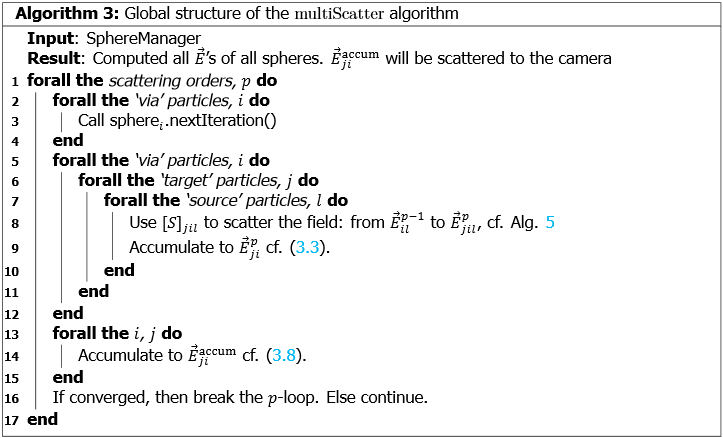
\includegraphics[height=0.6\textheight]{../figures/AlgorithmMScThesis.png}
\end{figure}
\tiny{Deze figuur komt uit mijn master afstudeerproject: http://www.kevinvanas.nl/TUDelft/MSc/Report.pdf}
}

\end{frame}


\begin{frame}
\frametitle{Wat is een algoritme?}

%TODO

\end{frame}


\begin{frame}
\frametitle{Wat is pseudocode?}
\framesubtitle{Oefening}

TODO: Oefening in de klas
%TODO

\end{frame}




